% R3b, RECAST AS A TIGHTNESS RESULT.  Session S4 wave 1, agent K2.
%
% S4 WAVE 4: the li2025o2cp citation below is wrapped in \mbox BECAUSE IT MUST NOT BREAK
% ACROSS A PAGE.  pdftex cannot split a hyperref link over a page boundary -- it dies with
% "! This can't happen (pdfvlistout)" after a \pdfendlink nesting warning -- and after this
% wave's edits the page 2/3 break landed inside "Li et al. [2025, Corollary 2]".  Do not
% remove the \mbox without rebuilding and checking the page break.
%
% S4 WAVE 2 (orchestrator): the mandated L1/L2 finding sentence appeared TWICE after
% wave 1 -- K1 put it in sections/setup.tex, where L1 and L2 are defined and where the
% qhat = -b/2 clause sits in the same breath, and K2 put a second copy in the tightness
% paragraph below.  The setup.tex instance is kept and this copy is CUT.  Frees 2 body
% lines, returned to this wave's reflow budget.
%
% ORDER IS LOAD-BEARING AND IS THE WHOLE POINT OF THE REWRITE.
%   (a) li2025o2cp Corollary 2's RETENTION result is stated FIRST and belongs to
%       its authors.  It is the thing being tested, not a caveat on this paper.
%   (b) this paper exhibits ONE legal perturbation -- the L1 dead band on the
%       COMPLETED threshold -- that leaves the admissible radius, and locates the
%       edge: tau* = sup_x r_t(x) + sup_t qhat_t - b/2.
%   (c) the condition is therefore TIGHT there, i.e. NECESSARY and not merely
%       sufficient.  That is a SMALLER and MORE PRECISE claim than "smoothing
%       forfeits the rate" and it is stated without hedging against that larger
%       claim.  Elsewhere the condition stays sufficient only, and the paragraph
%       says so: that asymmetry is what makes "tight" a LOCATED claim.
%
% MOVED IN FROM sections/limitations.tex THIS WAVE.  The saturator-level-4b
% result and ACT23's tangent-integrator result sat in the concession list, where
% they read as unexplained caveats ("the headline collapses to 20.10 and nothing
% explains why").  They are the SAME mechanism as the scorecaster sweep --
% sup r_t and sup qhat are the two terms of tau* -- so they are part of the
% CHARACTERISATION and belong inside it.  limitations.tex loses those lines and
% this section gains them; the exchange is recorded in both headers.
%
% EVERY NUMBER IN THIS SECTION TRACES TO A results/ JSON (docs/GATES.md G7.1):
%   primary       results/forfeit-20260820T063045Z-83747c45.json
%   tau-cliff     results/forfeit-20260820T063132Z-83747c45.json
%   variations    results/forfeit-variations-20260820T101445Z.json
% Row-by-row trace, one row per printed number with file + JSON key path + value:
% research/S4/K2-tightness.json, field number_trace.  Code: src/forfeit.py,
% src/test_forfeit.py.
%
% S5 SUB-SESSION A (2026-08-20): NUMERIC PROVENANCE AUDIT.  All 66 Table 1 cells were
% re-derived from results/forfeit-20260820T063045Z-83747c45.json, aggregate_table, regime
% == "adversarial", and every one agrees to printed precision.  Four changes here:
%   (a) TABLE 1 GAINED "miscov. 10^6" (aggregate_table[*].miscoverage at T = 1e6), because
%       the abstract cited arm ema_w0.999's 0.100004 and the table had no 10^6 miscoverage
%       column to check it against.  Seven columns fit with 0 overfull boxes.
%       AMENDED S5 WAVE 6 (J1): THE ABSTRACT NO LONGER PRINTS 0.100004.  Wave 3's rewrite
%       dropped the 42x / T = 1e6 / 0.100004 group AS A UNIT, deliberately, so the
%       miscoverage figure could not be re-paired with the wrong horizon a second time.
%       The COLUMN stays and is right -- all eleven values re-derived twice, and it is what
%       makes the T = 1e6 arm checkable at all -- but the BOLD on 0.100004 no longer points
%       at an abstract sentence.  It is kept because the body still turns on that arm
%       (61.08 -> 42.10, travel 28,311 -> 202), i.e. it now marks what SECTION 3 discusses
%       rather than what the abstract quotes.  Recorded so nobody re-derives the reason.
%   (b) "the ratio falls with the horizon, 61.08 to 42.10" NAMED NO ARM AND NO HORIZONS, and
%       the sentence had just said "for the last two" (w = 0.99 AND w = 0.999).  61.08 and
%       42.10 are ema_w0.999 ALONE, at T = 1e4 and T = 1e6 (aggregate_table[16] and [19],
%       ratio_max_abs_E_over_bound).  Both are now named.  The flatness claim itself is
%       correct for both arms: max_abs_E is 63.00 at all four horizons for w = 0.99 and
%       623.70 at all four for w = 0.999.
%   (c) "623.70 falls to 20.10" -- 623.70 is flat in T but 20.10 is NOT (13.80/17.00/17.90/
%       20.10 across the four horizons, rows[192..195]), so the horizon is now stated.  Same
%       for the tangent tau = 1.5 miscoverage 0.100001 (rows[207]).
%   (d) "tau = 2.0, 2.5, 3.0 and 5.0 fail too" sat immediately after a T = 10^6 figure but
%       those four bands were only ever run at T = 2x10^5 (variation wide_deadbands_baseline,
%       rows[225..228]).  The horizon is now stated.
%   Also fixed: "Every dead-band dead-band configuration" -> one "dead-band".
% VERIFIED UNCHANGED, no edit needed: 70.80 is arm ema_w0.999, regime EXACT_THRESHOLD_STRICT,
% flat across all four horizons (aggregate_table[104..107].max_abs_E) -- which is exactly the
% regime the sentence describes ("playing the threshold exactly ... under the same indicator,
% because its signature move then covers").  The 6.30/63.00/623.70 triple is read off the
% actual T = 1e4 rows (aggregate_table[8], [12], [16]), not inferred from the 1e6 column.
% The 19-of-19 law check re-ran clean: 15 at T = 1e6 over five settings x three widths, plus
% 4 wide bands at T = 2e5, 0 mismatches.  "its realised supremum is b - tau to the printed
% digit at every tau >= 0.9" IS computable from results/: max(arms_raw[*].trace.q_deployed)
% equals b - tau to nine decimals at every one of the ten grid widths >= 0.9, and is 1.2203
% (< 1.5) at tau = 0.5, so the ">= 0.9" qualifier is exactly right.
%
% S4 WAVE 2 (orchestrator): TABLE 1 NOW LISTS ALL ELEVEN ARMS.  The two S3 wave 5 dropped
% to pay for the boundary-law correction -- "partial adj. w = 0.5" and "growing time
% constant p = 0.5" -- are RESTORED from results/forfeit-20260820T063045Z-83747c45.json
% (aggregate_table, arms ema_w0.5 and growing_ema_p0.5, regime adversarial, T = 2e5 and
% 1e6).  Both cover and both sit inside the bound, so restoring them removes a disclosure
% caveat rather than adding evidence.  Prose counts updated nine -> eleven.  Also restored,
% because the resize freed the space K2 had to compress them into: the T = 10^4 excursion
% triple, the anti-windup mechanism sentence, and the tie-rule sentence.
%
% SUPERSEDED NOTE, kept for the record:
% TABLE 1 LISTS NINE OF THE ELEVEN ARMS RUN.  "partial adj. w = 0.5" (0.100030,
% 7.70, 0.52, 0.0000, 18,113) and "growing time constant p = 0.5" (0.100030,
% 12.60, 0.85, 0.0000, 330) were dropped in S3 wave 5 to pay for the boundary-law
% correction.  Both COVER and both sit inside the bound, so nothing adverse is
% hidden; every count in the prose is stated against the nine that are listed.
% The table is UNCHANGED this wave.
%
% WAVE-5 CORRECTION, CARRIED (S3 F1, research/S3/F1-adversarial.json 0-4).  An
% earlier version printed "coverage survives if and only if tau <= b/2" and "the
% failing set is (b/2,b]".  Both are false as general statements.  b/2 is the
% value of tau* at the NULL scorecaster and the MINIMAL admissible saturator; a
% legal constant scorecaster moves it, and the failing set is unbounded above.
%
% S4 CORRECTION, G7.1: "coverage survives to tau = b" IS DELETED.  It was printed
% of the qhat = +b/2 arm, where tau* = b, but no dead band of width b was ever RUN
% at that scorecaster -- the widths run there are 0.5, 0.9 and 1.5.  The sentence
% was a prediction from the law wearing the clothes of a measurement.  Replaced by
% the measurement: every width run at +b/2 covers, tau = 1.5 at 0.100010.
%
% S4 CORRECTION, G7.1: "31 OF 32 GRID POINTS" IS NOT PRINTED.  docs/GATES.md
% G7.9, docs/OUTSTANDING.md O52 and docs/S3_REPORT.md sec. 2 all carry it, and
% all three rest on ONE line in research/S3/patch-log.json -- an S3 orchestrator
% assertion in a gitignored file.  Neither the 32 points nor the unresolved one is
% identified anywhere, and no 32-point grid is reconstructible from results/.  A
% number that cannot be traced is deleted, not footnoted.
%
% WHAT IS PRINTED INSTEAD, AND IT IS FULLY TRACEABLE.  Applying tau* = sup_x
% r_t(x) + sup_t qhat_t - b/2 (b = 2, and sup_x r_t(x) = saturator_level_mult * b
% by src/forfeit.py:306) to every dead-band configuration in
% results/forfeit-variations-20260820T101445Z.json and comparing the predicted
% verdict with the measured miscoverage: 15/15 at T = 10^6 over the five
% (saturator, scorecaster) settings (baseline, qhat = +b/2, qhat = -b/2, level 4b,
% ACT23 tangent) at tau = 0.5/0.9/1.5, plus 4/4 on the wide bands tau =
% 2/2.5/3/5 at T = 2e5 -- 19 OF 19, NO COUNTEREXAMPLE.  Verified independently by
% K2; the arithmetic is in research/S4/K2-tightness.json (law_check_19_of_19).
% results/forfeit-20260820T063132Z-83747c45.json adds 11 more widths at the
% baseline setting, also 11/11, and is NOT folded into the printed count.
% The resolution caveat -- three widths per setting bracket each edge rather than
% locate it -- and the run that would close it are printed in the same sentence.
%
% FRAMING sec. 3: every quantifier is a measurement; no forbidden construction.
% The endpoint COVERS, so "tau > tau*" is the failing condition and writing
% "tau >= tau*" would be wrong.

\section{The edge of the admissible set, measured}
\label{sec:forfeit}

\begin{table}[tb]
\centering
\scriptsize
\setlength{\tabcolsep}{4.5pt}
% S5 wave 4: arraystretch 0.95.  Eleven data rows at 0.95 give back one typeset line,
% which was two of the last two lines standing between the body and the 4-page ceiling.
% This is row LEADING only -- no font change, no row removed, no cell altered.
\renewcommand{\arraystretch}{0.95}
% S6 SUB-SESSION B: CAPTION REWRITTEN TO DESCRIBE ONLY.  Two clauses left, and neither
% was deleted:
%   "so no covering arm is withheld" was a REBUTTAL, not a description.  The fact it
%     defended -- that every arm run appears -- is still the caption's first sentence.
%   "five exceed the bound at T = 10^6" was a CONCLUSION about the data, and it existed
%     NOWHERE ELSE in the paper (grepped: one hit, this caption).  It moved into the
%     retention paragraph below, where Table 1 is first discussed.  Independently
%     recounted from the table's own ratio column: 4.25, 42.10, 3.58, 3.34 and 60,747
%     exceed 1, so five is right.
\caption{Placement~A: a one-scalar readout on the \emph{completed} threshold, under one
deterministic adversary, on one pass to $T = 10^6$; all eleven arms run are listed.
Proposition~2's bound is $13.2061$ at $T = 2{\times}10^5$ and $14.8155$ at $T = 10^6$;
``ratio'' is $\max_t|E_t|$ over it, and ``Sat.'' the fraction of rounds on which~(4)
delivers its full $\pm b$. Every number is the \emph{primary} regime's, defined in
Appendix~\ref{app:support}, which also gives the $T = 10^4$ excursions and the fitted
excursion law.}
\label{tab:forfeit}
\begin{tabular}{@{}lrrrrrr@{}}
\toprule
Readout on the completed threshold & miscov.\ $2{\times}10^5$ & miscov.\ $10^6$ &
$\max_t|E_t|$ $10^6$ & ratio & Sat.\ $10^6$ & travel $10^6$ \\
\midrule
none (control)                & $0.100035$ & $0.100007$ & $7.80$        & $0.53$     & $0.0000$ & $28{,}311$ \\
partial adj.\ $w = 0.5$       & $0.100030$ & $0.100007$ & $7.70$        & $0.52$     & $0.0000$ & $18{,}113$ \\
partial adj.\ $w = 0.9$       & $0.100030$ & $0.100007$ & $7.50$        & $0.51$     & $0.0000$ & $4{,}081$ \\
partial adj.\ $w = 0.99$      & $0.100040$ & $0.100006$ & $63.00$       & $4.25$     & $0.0007$ & $1{,}023$ \\
partial adj.\ $w = 0.999$     & $0.100035$ & $\mathbf{0.100004}$ & $623.70$      & $42.10$    & $0.0097$ & $202$ \\
growing time constant $p=0.5$ & $0.100030$ & $0.100006$ & $12.60$       & $0.85$     & $0.0000$ & $330$ \\
growing time constant $p=0.9$ & $0.100030$ & $0.100024$ & $53.00$       & $3.58$     & $0.3181$ & $16$ \\
running mean                  & $0.099940$ & $0.100010$ & $49.50$       & $3.34$     & $0.3647$ & $9$ \\
dead band $\tau = 0.5$        & $0.100035$ & $0.100005$ & $10.60$       & $0.72$     & $0.0000$ & $2{,}045$ \\
dead band $\tau = 0.9$        & $0.100060$ & $0.100012$ & $13.20$       & $0.89$     & $0.0038$ & $1{,}051$ \\
dead band $\tau = 1.5$        & $\mathbf{1.000000}$ & $\mathbf{1.000000}$ & $900{,}000$ & $60{,}747$ & $1.0000$ & $0.5$ \\
\bottomrule
\end{tabular}
\end{table}

\paragraph{The retention result is published, and tested from outside.}
\mbox{\citet[Corollary~2]{li2025o2cp}} prove that a predictable $d_t$ with $|d_t| \le
\mu_t(b/2-|\hat{q}_t|)$ on the deployed threshold keeps (\ref{eq:pid}) in error-integration form
and \emph{retains} $|E_T| \le c\,h(T)+1$: the radius is theirs. A downstream partial
adjustment of weight $w$ leaves it; Table~\ref{tab:forfeit} prices that departure, and five of its
eleven arms exceed the bound at $T = 10^6$. For $w = 0.99$ and
$0.999$ the excursion is \emph{flat in $T$} while the bound grows like $\log T$. At $w = 0.999$
the ratio is $61.08$ at $T = 10^4$ and $42.10$ at $T = 10^6$. The
forfeit is a property of the smoothing \emph{strength}, not Placement~A, and it buys something:
travel falls from $28{,}311$ to $202$. The forfeit's sign is counter-intuitive. A readout on the completed
$q_{t+1}$ touches neither $r_t$ nor the integrator's argument, so it cannot put~(4) at risk. It delays a
correction already computed, and the accumulator excurses
\emph{further}. Smoothing the output does not damp $E_t$; it feeds it. That $623.70$ turns on the
adversary's $\varepsilon$, not the counting convention.

% ---------------------------------------------------------------------------
% S5 WAVE 2: sub-session B's boundary figure, inserted here.
% It is referenced by \ref{fig:boundary} from the paragraph immediately below.  It
% appears AFTER the schematic in document order, so LaTeX typesets it as Figure 2.
%
% S6 SUB-SESSION A: REBUILT.  Two measured defects drove it, both recorded in
% research/S6/A0-diagnosis.json and both re-measured against the RENDERED artefact
% rather than read off the generator:
%   (1) the old panel (b) placed the eleven-point grid by INDEX.  The located window
%       tau in [1, 1.001] took 10.000% of that axis while being 0.0910% of the true log
%       span: inflated x109.9, which erased the one thing the grid was run to show.  It
%       is now placed by tau - tau* on matplotlib's native SYMLOG scale, linthresh 1e-3.
%   (2) panel (a) carried five settings, five tau* markers in three styles, two inline
%       annotations and a legend.  Four markers nested at (tau=0.5, miscov~0.1) and the
%       legend frame overwrote 627 px of the tau*=1 rule and 651 px of the tau*=2 rule
%       (pixel diff, legend drawn vs not drawn, 400 dpi).  Panel (a) now carries ONE
%       setting: the null scorecaster, the only one with runs on both sides of its own
%       tau*.  The five-setting comparison moved to Figure~\ref{fig:settings} in
%       Appendix~\ref{app:support}, where a categorical axis can do it properly.
% NOT A DEFECT, recorded because the S6 brief asserted it was one: panel (a)'s x-axis was
% ALREADY log-scaled under S5.  Its rendered tick positions matched true log positions to
% 1.1e-16 and the gap-by-gap distortion factor was exactly 1.000 at all six gaps.
%
% Built by src/make_figure1.py, which reads results/ directly and whose check_law() and
% check_grid_law() re-derive tau* per setting and test it against every measured
% miscoverage, exiting non-zero on any inconsistency -- so neither figure can be produced
% from data that contradicts the law it draws.  Its overlap_audit() then fails the build
% on any two text or legend boxes that come within 1.6pt of each other.  The generator
% pins CreationDate, so re-running it reproduces both PDFs byte for byte.
% THE CAPTION CARRIES NO EM-DASH.
% ---------------------------------------------------------------------------
\begin{figure}[tb]
  \centering
  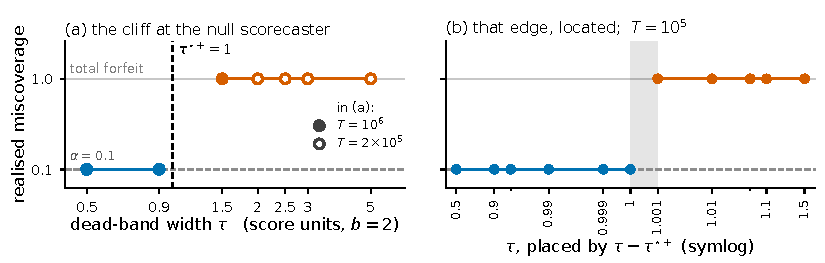
\includegraphics[width=\textwidth]{figures/figure1_boundary.pdf}
  \caption{Realised miscoverage against dead-band width $\tau$ at the null scorecaster,
  $\hat{q} \equiv 0$ with a saturator of level $b$, where $\tau^{\star} = \sup_x r_t(x) +
  \sup_t \hat{q}_t - b/2$ is $1$. \textbf{(a)} The full sweep: filled markers run to
  $T = 10^{6}$ and the four widest bands, drawn open, to $T = 2{\times}10^{5}$; blue
  covers, orange forfeits, and the dashed rule is $\tau^{\star}$. \textbf{(b)} The same
  setting at $T = 10^{5}$ over eleven measured widths, placed by $\tau - \tau^{\star}$ on
  a symlog axis whose linear zone is $|\tau - \tau^{\star}| \le 10^{-3}$, which magnifies the
  neighbourhood of $\tau^{\star}$: visual spacing here is not proportional to true distance in
  $\tau$. Unlabelled minor ticks mark $\tau = 0.95$ and $1.05$. The grey band spans the widest covering width to the
  narrowest failing one; Figure~\ref{fig:settings} gives the other four $(r_t,\hat{q})$
  settings.}
  \label{fig:boundary}
\end{figure}

\paragraph{The $L_1$ dead band leaves the radius, and the edge is measurable.} A dead band pulls
the deployed threshold back by exactly $\tau$ when it releases, so ``inside Corollary~2'' reads
$\tau \le \mu_t(b/2-|\hat{q}_t|)$. Under saturation the deployed value is pinned $\tau$ below the
integrator's ceiling, and its realised supremum is $b-\tau$ to the printed digit at every $\tau \ge
0.9$. The adversary's best legal play is $b/2$, so coverage is lost when that supremum drops below
it, at $\tau^{\star} = \sup_x r_t(x) + \sup_t \hat{q}_t - b/2$. All $19$ dead-band
runs agree with that law (Figure~\ref{fig:settings}); only the null scorecaster's edge is located
(Figure~\ref{fig:boundary}), the others one-sided. \textbf{Here $\sup_x r_t(x) = b$ and $\hat{q} \equiv 0$, so
$\tau^{\star} = b/2$}, one point of the admissible class, and both terms move it. The legal
$\hat{q} \equiv +b/2$ carries the $\tau = 1.5$ band inside the bound. The equally legal $\hat{q}
\equiv -b/2$ drops the edge to $0$, and there $\tau = 0.5$ returns $1.000000$, as does partial
adjustment at $w = 0.999$. Condition~(4) bounds $\sup_x r_t(x)$ only from below, so raising it
costs the theorem nothing; it moves the edge too (Figure~\ref{fig:settings}) and shrinks
the excursion. Under the unbounded tangent integrator
\citet{angelopoulos2023pid} report using in all their experiments, $\tau^{\star}$ is unbounded and
all three widths there cover. The excursion is $20.10$ rather than $623.70$, both at $T = 10^6$. \textbf{The method's own integrator therefore
sits inside the set at every width run here.} Outside the set the transition is a step. Past
$\tau^{\star}$ the threshold sits permanently below the reachable score range and $|E_t| =
(1-\alpha)t$ grows linearly, $60{,}747$ times the bound at $T = 10^6$. The wider bands $\tau =
2.0$, $2.5$, $3.0$ and $5.0$ fail too at $T = 2{\times}10^5$ (Figure~\ref{fig:boundary}), so the
failing set is $(\tau^{\star},\infty)$, open at the left. \textbf{The endpoint is where the adversary's
specification decides the answer.} At $\tau = \tau^{\star}$ the deployed supremum equals the
adversary's own cap $b/2$, so the clip forces an exact play and the reading settles it: the
primary regime covers. Appendix~\ref{app:support} separates the two readings and prints both.
\textbf{The failing arms have $\mathrm{Sat.} = 1.0000$.} Condition~(4) delivers its full
$\pm b$ on every round, and what fails is Proposition~2's other hypothesis: the threshold closing
the loop \emph{is} the integrator's output.

\paragraph{What that measures is that the published condition is tight.} At $\mu_t = 1$,
$\hat{q} \equiv 0$ the measured $\tau^{\star}$ is exactly Corollary~2's radius, and crossing it
costs coverage rather than the rate. \textbf{The claim is that necessity: a tightness result about
someone else's sufficient condition}, smaller and more precise than a forfeit of the rate by
post-processing. Elsewhere it stays sufficient only: at $\hat{q} \equiv +b/2$ Corollary~2
permits radius $0$ while every width run there covers. That asymmetry makes ``tight'' a located
claim.

\paragraph{The constructive reading, and it is the corollary's rather than ours.} Placement~B
keeps $\{\hat{q}_t\}$ inside the admissible radius, so Theorem~1 carries it already. What the
measurement adds is that the band has an edge, computable before deployment from $\sup_x r_t(x)$
and $\sup_t \hat{q}_t$, and that crossing it is not a graceful degradation.
